\subsection{Practices and standards}

In the previously mentioned process manual, some standards and practices, which the \glspl{devTeam} have to follow, are mentioned. These fit into the following categories:

\begin{itemize}
    \item Coding standards
    \item Documentation standards
    \item Version control
    \item Code review
\end{itemize}

The coding standards involve naming conventions, descriptions, and a few other aspects. This is done so the code is easier to read for people that need to get familiar with the system, mainly the future \glspl{devTeam}, because we found it hard to get to know the system when it was made by a lot of different people, with a lot of different coding standards.

Last year, the project and repository were moved to GitLab that takes care of the version control. At the beginning of this semester, our team moved it to Github. This is documented in \autoref{sec:GitAndCI}. The workflow of the project is done using GitFlow Workflow. The manual describes the rules for using branches. The point of the code review is to make sure that all code committed by the \glspl{devTeam} follow the coding standards. When a Team tries to merge code into production, two people from different groups have to review it. They have to go through a checklist (see \autoref{app:code-review-checklist}), to see if everything is all right.

Another decision made is, that the \glspl{devTeam} should document the implemented components, their responsibility and how it interacts with other components. This documentation should be stored in the wiki repository on the \gls{giraf} Github page. The wiki should ultimately contain all information needed to get to know the different components in the system.

If a member of a team finds an issue in the program, he can make an issue report. This makes it possible to document errors systematically, without the \glspl{team} having to fix it themselves. If a \gls{team} however finds it important to introduce a new task to the product backlog, the team can issue a task creation request. The \gls{POT} then decides if they find it relevant to have in the product backlog.

The process between the \gls{G19} \glspl{devTeam} is defined in the manual. This process will be evaluated at each \gls{SOSSprintRetrospective}, and changed as needed. It is designed to make the collaboration between the \glspl{team} run as smoothly as possible, without interfering with the \glspl{team} internal processes.

\subsubsection{Version Control}
Regarding version control a strict strategy was enforced, this was to ensure that all developers utilized the version control similarly. The strategy enforced was GitFlow \cite{GitFlow}. GitFlow is a Git Workflow design originally published by Vincent Driessen, the aim of GitFlow is to set a framework for managing large scale projects.

The way GitFlow achieve an easier management of large scale projects is in its strict branching rules. The framework dictates that a project should have the following branch types\cite{GitFlow}:

\begin{itemize}
    \item One master branch - this is the branch where the most recent release is, every commit to this branch is a new release.
    \item One develop branch - this is the branch where active development is merged into, it is based on the master branch. The develop branch is never merged into other branches.
    \item A set of feature branches - every feature should have its own branch, which is based on the develop branch and should merge back into the develop branch when it is finished.
    \item A set of release branches - when there are enough new features in the develop branch or when a new release is scheduled. A release branch is forked out of the develop branch. This branch is not allowed to have any feature-branches merged into it, only bug fixes. When the release branch is stable it is merged into master and thereby becoming the newest release.
    \item A set of hotfix branches - If a bug is revealed in the current master branch a hotfix branch should be created, this is forked off the master branch and should be merged with both the master and develop branch.
\end{itemize}

This framework was adopted into the \gls{giraf} Project\cite{ProcessGitFlow}. The biggest differences between the standard GitFlow framework and the \gls{giraf} adaptation are:

\begin{itemize}
    \item A feature branch is to be squashed and merged with the develop branch. This ensures every feature is only one commit in the develop branch.
    \item Release branches are forked off the master branch and all relevant features are cherry-picked from the develop branch. Cherry-picking is when one merges a specific subset of commits from one branch to another.
    \item Hotfixes are merged into the release branch.
    \item The release branch is merged into the master and develop branch.
\end{itemize}
\begin{figure}[H]
        \begin{center}
            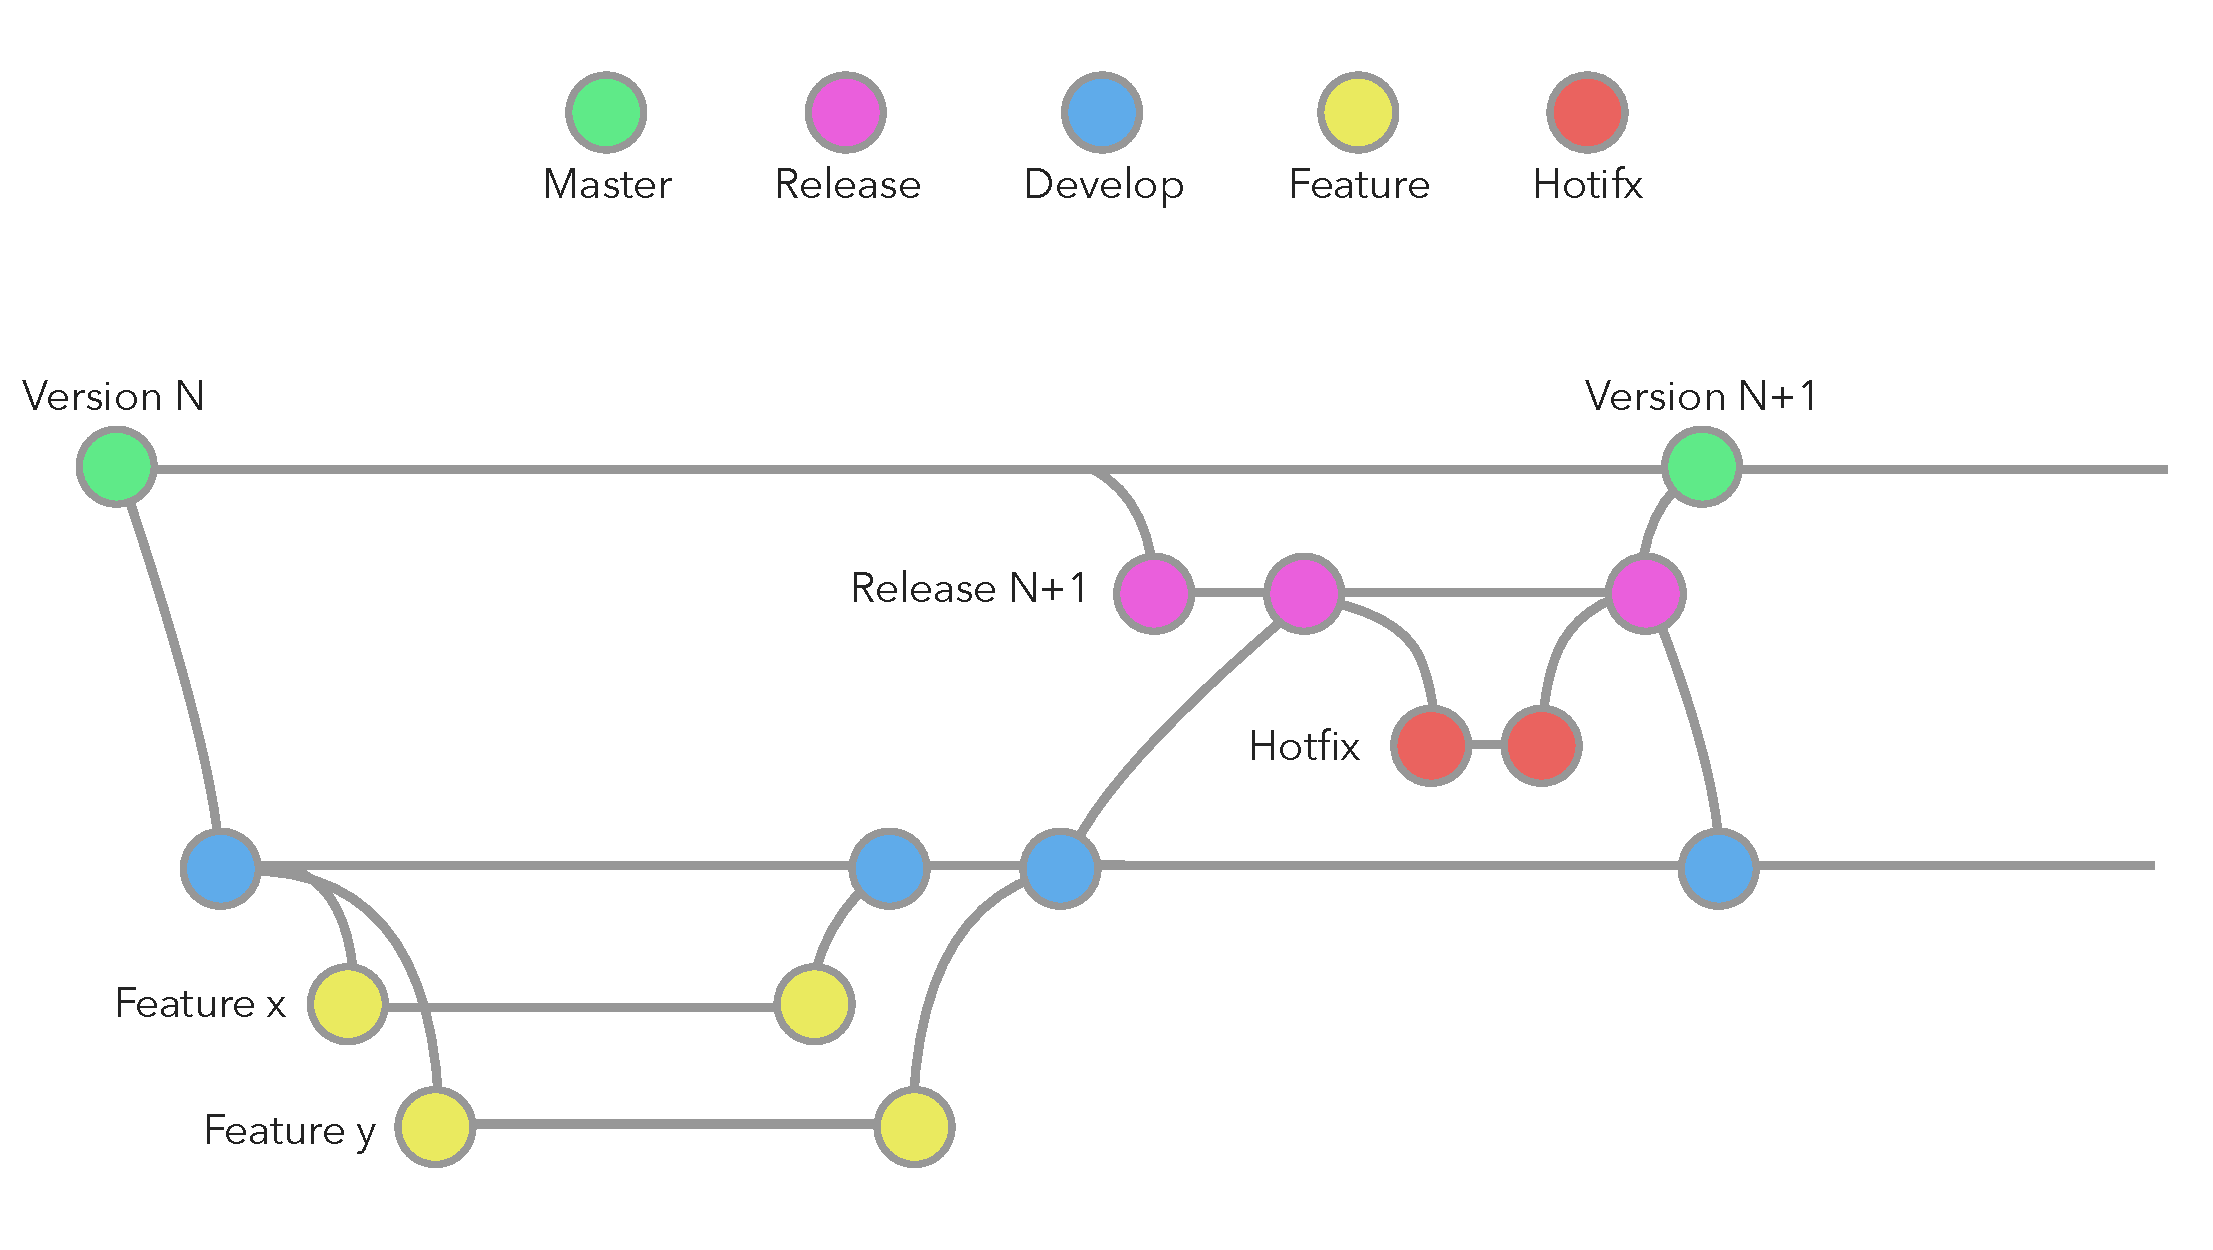
\includegraphics[width=0.95\textwidth]{figures/giraf_gitflow_illustration.pdf}
        \end{center}
        \caption{A illustration of the \gls{giraf} adaptation of GitFlow}
        \label{fig:girafgitFlowfigure}
\end{figure}
\autoref{fig:girafgitFlowfigure} illustrates the \gls{giraf} Adaptation of the GitFlow, in the illustration one can see how Feature y is cherry picked and Feature x is not.
